\documentclass[letterpaper,12pt]{article}
\usepackage[corrige]{examS2M} % Avec l'option corrige, les réponses apparaissent
% \usepackage[]{examS2M} % Sans l'option corrige, les réponses n'apparaissent pas
\usepackage{graphicx} 
\usepackage{caption}
\usepackage{textcomp}


\begin{document}

% Description de l'exam
\universite{Université de l'Univers}
\departement{Kinésiologie}

\typeExamen{Exemple}
\dateExamen{Le 30 février 42}
\sigleCours{KIN4242}
\nomCours{Biomécanique (ou autre)}
\nomProf{Machin truc 1 \& Machin truc 2}
\ponderation{50}
\entete

\begin{directives}
  \item Sacs et manteaux doivent être déposés en avant de la salle.
  \item Aucun étudiant ne peut sortir de la salle d'examen dans la première heure.
  \item Aucune permission ne sera accordée durant l'examen pour aller à la salle de bain.
  \item Signer la feuille de présence après avoir rendu sujet d'examen et feuillet réponse.
\end{directives}

\begin{autresInfos}

  \begin{tabularx}{\linewidth}{lXr}
    \hspace{-9px} L'examen est composé de : & & \\
    \total{NombreVraiOuFaux} questions vrai ou faux	& (Chaque question vaut \points{1}) & $/ 3$ \\
    \total{NombreChoixMultiples} questions à choix multiples	& (Chaque question vaut \points{2}) & $/ 4$ \\
    \total{NombreDeveloppement} questions à développement & (Pondération variable) & $/ 9$ \\
  \end{tabularx}
  
\end{autresInfos}





\begin{questions}
  
  % Exemple de question vrai ou faux
  \enteteSectionVraiOuFaux{1}
  
  \begin{vraiOuFaux}
    {Vrai ou faux?}
    {vrai}
  \end{vraiOuFaux}
  \begin{vraiOuFaux}
    {Encore un vrai ou faux?}
    {vrai}
  \end{vraiOuFaux}
  
  
  
  
  % Exemple de questions à choix multiple
  \enteteSectionChoixMultiples{2}

  % Question à choix multiple
  \begin{choixMultiples}{Qu'est-ce que l'importance?} 
      \reponse	Rien
      \reponse	Tout
      \bonneReponse Heu.. Wtf?
  \end{choixMultiples}
  
  % Question choix multiple différente, utiliser la commande \reponse pour faire apparaitre la réponse si souhaité
  \begin{customQuestion}{Une question choix multiple avec un layout fucked up.}{choixMultiples}
  \centering 
    { % À noter que includegraphics peut être utilisé directement dans choixMultiples également
      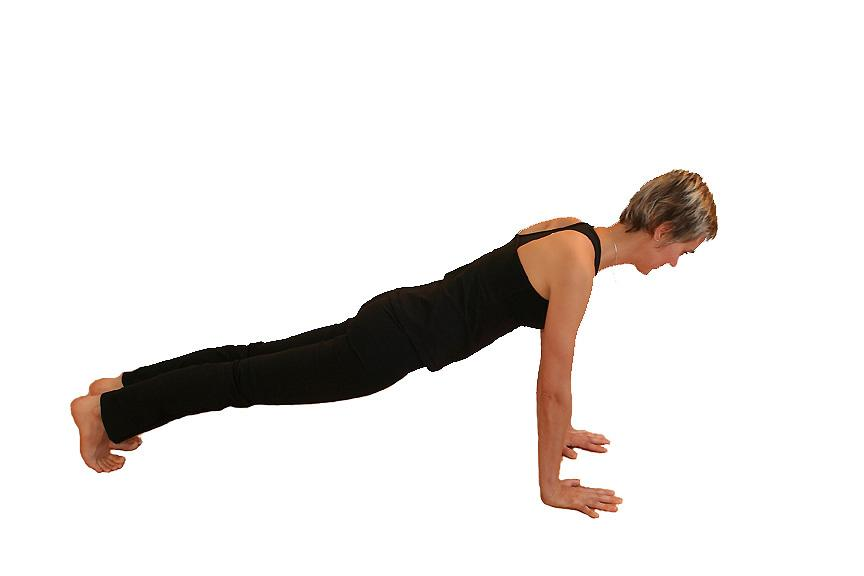
\includegraphics[width=.2\linewidth]{figures/uneImage.jpg}
      \captionof{figure}{Une figure importante à la question.}
      \label{fig:uneImage}      
    }
    \vspace{15px}
    \begin{minipage}{.4\linewidth}
      \begin{enumerate}
       \reponse	Ligne 1
       \reponse	Ligne 2
       \reponse	Ligne 3
      \end{enumerate}
    \end{minipage}
    \hspace{15px}
    \begin{minipage}{.4\linewidth}
      \begin{itemize}
       \renewcommand\labelitemi{\rule{30px}{1px}}
       \reponse	\bonneReponse{(B)} L'autre ligne 2
       \reponse	\bonneReponse{(A)} L'autre ligne 1
       \reponse	\bonneReponse{(C)} L'autre ligne 3
      \end{itemize}
    \end{minipage}
  \end{customQuestion}


  \begin{vraiOuFaux}
    {Vrai ou faux, mais sans en-tête?}
    {vrai}
  \end{vraiOuFaux}
  
  
  % Exemples de questions à développement
  \enteteSectionDeveloppement
   
  % Question valant 4 points à expliquer sur 8 lignes
  \begin{Developpement}{Pourquoi? (\points{4})}{8}
    \bonneReponse{Ceci est LA réponse : 42}
  \end{Developpement}

  % Question valant 5 points dont le layout est au choix du professeur
  \begin{customQuestion}{Non, mais pourquoi? (\points{5})}{Developpement}
	Fait/Dessine ce que tu veux ici!  
	
	\bonneReponse{Mais la bonne réponse demeure 42}
   \end{customQuestion}
   
  
\end{questions}

\end{document}
